\documentclass[a4paper, 12pt]{article}
%\usepackage{enumerate}
\usepackage{graphicx}
 \usepackage{url} % allow url in bibtex
\usepackage{float} % force picture to place [H] HERE

 \usepackage{graphicx} %load package for graphic
  \usepackage{subcaption} % two figure side by side
 
 \usepackage{indentfirst} % indent the first paragraph in section
 
\title{CS412 - Report 1\\ Face expression recognition (1)}
\date{\today}

\begin{document}

\begin{center} 
\large VNUHCM - University of Science\\
Faculty of Information Technology\\
Advanced Program in Computer Science
\end{center}

\begingroup
\let\newpage\relax
\maketitle
\endgroup

\textbf{Group members:}
\begin{enumerate}
	\item 1351040 : Thai Thien
	\item 1351059 : Ho Ngoc Huynh Mai
\end{enumerate}

\section{Introduction}

We choose to do Face expression recognition. Our implement will based on paper Robust Facial Expression Classification Using Shape and Appearance Features of SL Happy and Aurobinda Routray \cite{7050661}. We adopt the preprocessing process, the feature extraction. But we do not intend to work on extract active patches. For the model, we plan to implement 2 model, a Support Vector Machine (as in \cite{7050661}) and a simple Neural network.      

\section{Project Details}
The purpose of this project is implement the system to recognize facial expression, including, but not limited to anger, disgust, fear, happiness, sadness and surprise. \\
Input: A face of someone. \\
Output: The facial expression. \\ 

\section{Methodology}

\subsection{Preprocessing}

\subsubsection{Gaussian blur}
By default, Opencv load image with BGR channel. We convert image to grayscale. Then apply Gaussian Blur with kernel size 5x5 and $\sigma$ = 1 to filter out noise.

\subsubsection{Face Detection}
The purpose of this step is to detect the face in input image. We use image which is smoothed from the step above as input for face detection. We use Haar feature-based cascade classifiers \cite{viola2001rapid} for face detection.

We use pre-trained data provided by OpenCV haarcascade\_frontalface\_default.xml. 

\subsubsection{Extract and resize}
We create the region of interest (ROI) from the face position detected by Haar classifiers. We create new image from region of interest and resize the image to 96x96.

\subsubsection{Result}

\begin{figure}[H]
	\centering
	\begin{subfigure}[b]{0.4\textwidth}
		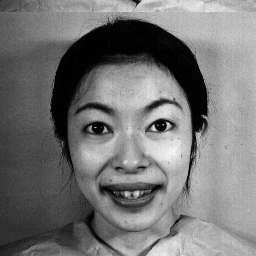
\includegraphics[width=0.9\textwidth]{./raw/img1.png}
	\end{subfigure}
	%
	\begin{subfigure}[b]{0.4\textwidth}
		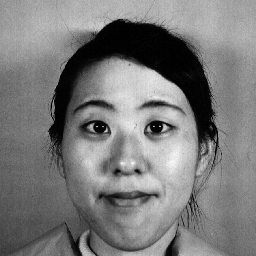
\includegraphics[width=0.9\textwidth]{./raw/img2.png}
	\end{subfigure}
	\caption[]{Before preprocessing}
	\label{fig:beforepre}
\end{figure}

\begin{figure}[H]
	\centering
	\begin{subfigure}[b]{0.4\textwidth}
		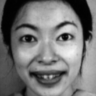
\includegraphics[width=0.9\textwidth]{./processed/img1.png}
	\end{subfigure}
	%
	\begin{subfigure}[b]{0.4\textwidth}
		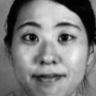
\includegraphics[width=0.9\textwidth]{./processed/img2.png}
	\end{subfigure}
	\caption[]{After preprocessing}
	\label{fig:afterpre}
\end{figure}



\subsection{Feature selection}
	This step we select feature to represent image. 
	For basic level, we try to implement the basic feature selection base on Open CV tutorial, such as Harris Corner Detection, Shi-Tomasi Corner Detector, Good Features to Track. 
	Then, we try to implement Local binary patterns (LBP) and pyramid of histogram of gradients (PHOG). 
	
\subsection{The model}
	The model is a classifier model, which take feature vector as a input and output the class it belong to. There are 6 classes anger, disgust, fear, happiness, sadness and surprise.
	
	For basic level, we implement a neural net, multi-layer perceptrons as the tutorial \cite{mlp}.
	
	Then, we implement the One-Against-One Support Vector Machine. We need total 15 OAO SVM for 6 classes.
	

\section{Data, Scenarios, and Models}
Dataset: Cohn-Kanade (CK and CK+) \cite{5543262}, jaffe \cite{lyons1998japanese}



\bibliographystyle{ieeetr}
\bibliography{Bibtex}

\end{document}

